\documentclass[12pt,fleqn]{report} %taille de la police par défaut, et équations jusitifées à gauche
\usepackage[left=2cm,right=2cm,top=2cm,bottom=2cm,headsep=10pt,a4paper]{geometry}
\usepackage{xcolor}
\definecolor{enstabGreen}{HTML}{C8D200} 	%vert  	#c8d200 
\definecolor{enstabLightGreen}{HTML}{E9ED99} 	%vert  	#c8d200 
\definecolor{enstabLightBlue}{HTML}{009EE0} %bleu clair 	#009ee0
\definecolor{enstabVeryLightBlue}{HTML}{99D8F3} %bleu clair 	#009ee0
\definecolor{enstabDarkBlue}{HTML}{005C8F}	%bleu foncé 	#005c8f
\definecolor{enstabDarkGrey}{HTML}{333333}	%gris fort 	#333333
\definecolor{enstabLightGrey}{RGB}{48,48,48}	%gris fort 	#333333
\definecolor{enstabParme}{HTML}{8878B2}		%parme 	#8878b2
\definecolor{enstabOrange}{HTML}{F18E00} 	%orange 	#f18e00
\usepackage[colorlinks=true,
        urlcolor=enstabLightBlue,
        anchorcolor=enstabDarkBlue,
        linkcolor=enstabDarkBlue,
        citecolor=enstabDarkGrey,
        pdfauthor={O. Reynet},
        pdfkeywords={LaTeX; Report},
        pdftitle={How to produce a report with LaTeX},
        pdfsubject={yours !}] {hyperref}
\usepackage{url}
\usepackage[utf8]{inputenc} % lettres accentuées
\usepackage[T1]{fontenc}    % Use 8-bit encoding that has 256 glyphs
\usepackage[UKenglish]{babel} % Pour le français
\usepackage{eso-pic}        % pour une image en fond, page de titre
\usepackage{graphicx}       % Pour inclure des images
\graphicspath{{images/}}    % Où sont les images ?

\usepackage{listings}      % Pour coloriser les codes que vous insérez
\lstset{ %
  backgroundcolor=\color{white},   % choose the background color; you must add \usepackage{color} or 
  basicstyle=\footnotesize\ttfamily,        % the size of the fonts that are used for the code
  breakatwhitespace=false,         % sets if automatic breaks should only happen at whitespace
  breaklines=true,                 % sets automatic line breaking
  captionpos=b,                    % sets the caption-position to bottom
  commentstyle=\color{enstabOrange},    % comment style
  deletekeywords={...},            % if you want to delete keywords from the given language
  escapeinside={\%*}{*)},          % if you want to add LaTeX within your code
  extendedchars=true,              % lets you use non-ASCII characters; for 8-bits encodings only, does not work with UTF-8
  %frame=single,                    % adds a frame around the code
  keepspaces=true,                 % keeps spaces in text, useful for keeping indentation of code (possibly needs columns=flexible)
  keywordstyle=\color{enstabDarkBlue},       % keyword style
  %language=Octave,                 % the language of the code
  morekeywords={*,...},            % if you want to add more keywords to the set
  numbers=left,                    % where to put the line-numbers; possible values are (none, left, right)
  numbersep=8pt,                   % how far the line-numbers are from the code
  numberstyle=\tiny\color{enstabDarkGrey}, % the style that is used for the line-numbers
  rulecolor=\color{black},         % if not set, the frame-color may be changed on line-breaks within not-black text (e.g. comments (green here))
  showspaces=false,                % show spaces everywhere adding particular underscores; it overrides 'showstringspaces'
  showstringspaces=false,          % underline spaces within strings only
  showtabs=false,                  % show tabs within strings adding particular underscores
  stepnumber=5,                    % the step between two line-numbers. If it's 1, each line will be numbered
  stringstyle=\color{enstabParme},     % string literal style
  tabsize=2,                       % sets default tabsize to 2 spaces
  title=\lstname                   % show the filename of files included with \lstinputlisting; also try caption instead of title
}





\usepackage{booktabs}       % pour de jolis tableaux
%\usepackage{fancyhdr}       % pour des entêtes et pieds de pages améliorés.
\usepackage{makeidx}        % requis pour faire les index
\usepackage{amsmath}
\usepackage{amsfonts}
\usepackage{amssymb}
\usepackage{color}
\usepackage{array}
\usepackage{graphicx}
\usepackage{caption} 
\usepackage{hyperref}
\usepackage{algorithm}
\usepackage{algorithmic}
\usepackage{times}
\usepackage{tabularx}     % Ce fichier contient tous les packages nécessaires à la compilation
\makeindex           % donne l'ordre de créer l'index

\begin{document}
\renewcommand{\contentsname}{Contents}                % des jolis noms pour la table des matières
\renewcommand{\bibname}{Bibliography}  % des jolis noms pour les sections bibliographiques

%----------------------------------------------------------------------------------------
%	 PAGE DE TITRE
%-----------------------------	-----------------------------------------------------------

\begingroup
\thispagestyle{empty}
\AddToShipoutPicture*{\put(6,5){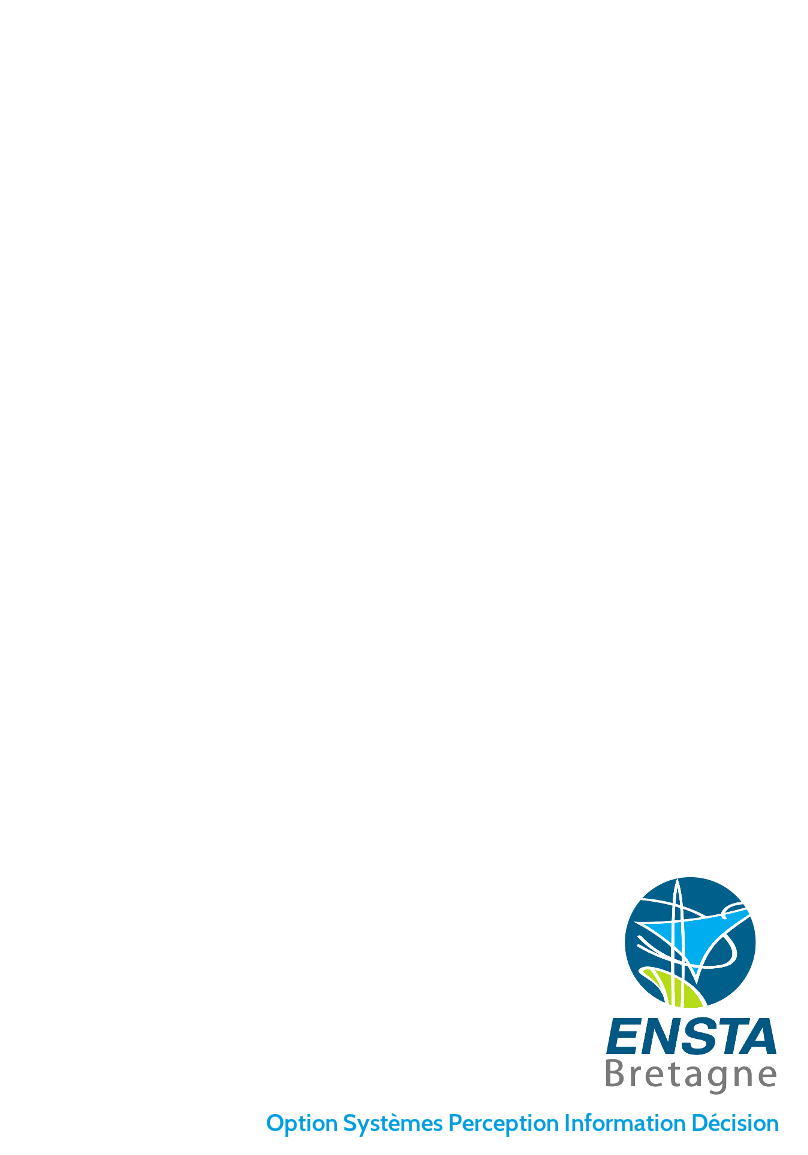
\includegraphics[scale=1]{Images/FondTitreSPID}}} % Image background
\begin{center}
\vspace*{2cm}
{\Huge \textsc{\textbf{Status Report}}}\\


\vspace*{2cm}
{\huge Time Frequency representation deformation}\par % Intitulé du projet
\end{center}
%\begin{figure}[H]
%\centering
%    \includegraphics[trim={1cm 1cm 0.7cm 5cm},clip, scale=0.6]{biscay.png}
%\end{figure}

\vspace*{1.5cm}
\textbf{\large Written by:} 
\begin{center}
{\large
\begin{tabular}{cc}
\\
\\
\\
Philippe Chuzel\\
\\
\\
\end{tabular}}
\end{center}


\vspace*{1.5 cm}
{\large \textbf{Under the supervision of:}}\\
\begin{center}
{\large
Jean-Christophe Cexus\\
Arnaud Coatanhay\\}
\end{center}
\endgroup


%----------------------------------------------------------------------------------------
%	SOMMAIRE
%----------------------------------------------------------------------------------------
\tableofcontents  % Imprime le sommaire
\cleardoublepage  % pour commencer sur une page impaire

\chapter*{Abstract}
This report has been made for the project TFR Deform which its purpose was to create a processing chain in order to analyse the electromagnetic field of object which its form change trough time. According to the recommendation of the supervisors, this project has considered only cylinder which its radius change through time. The deliverable wanted was:

\medskip

\begin{itemize}
\item Create a script which can provide the field scatter by the cylinder, the incident wave and all the geometric parameters of the simulation.
\item Implement or use different time frequency representation in order to see the modification of the electromagnetic signature of the object through time.
\item Implement methods in order to interpolate the law frequency of the electromagnetic signature and, if there was enough time, find correlation between those modifications and the deformation of those objects.
\end{itemize}

\medskip

In the end, the code for the generation of signal is working very well and, even if we implemented our own functions for the time frequency representation at the beginning of the project, we found a library which provide the same functions with a lot of other tools which provide a lot of help during the project. The modelization of the movement is also working and provide excellent result on the time frequency representation. Nevertheless, there are still some work to do in order to see the impact of the variation of the form of the object. The processing chain is working but it remains a little work in order to finalize the study of the signal.


\chapter*{Introduction}
The purpose of this project is to analyse the electromagnetic signature of object when its form changes during time. The electromagnetic signature analysis is a common subject for people who work in the filed of radar detection. However, the study of object signature which its form change through time is still full of many questions which have not been answered. The study of those object imply to do a very strict analyse of the electronic signature thanks to the time frequency analysis tools.

\bigskip

During this project \cite{Analysis}, we have to look at the different tools which can help us to analyse the electronic signature of an object and to help us to understand the effects of change of shape of an object. The final deliverable expected is a set of program which can allow us to implement an entire loop of treatment. This loop has to help us to understand how an object deformed according to the modification of its electronic signature. \textbf{All the code had to be done in python} which imply that some function had to be implemented by ourself. A lot of documentation have been given by the supervisor  but only have

\bigskip

The whole project code and result can be find here :

\textit{https://github.com/chuzelph-ENSTA-Bretagne/TFR \_ Deform.git}


\begin{figure}[H]
\centering
    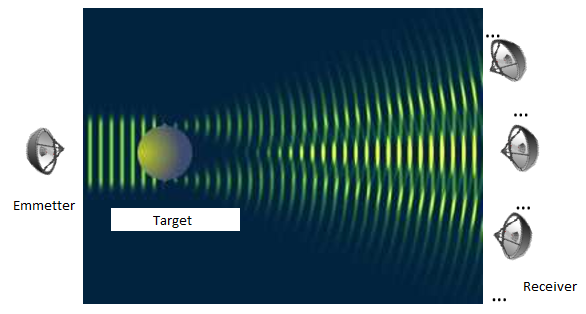
\includegraphics[scale=1,angle=0]{Images/Image1.PNG}
    \caption{General situation of our subject.}
    \label{fig:Image1}
\end{figure}

\bigskip

The first part will try to explain which equations have to be understood in order to get the analytic expression of the electromagnetic field coming from the object.
The second part will expose the different tools which have been create for the time frequency analysis that can be used for this project. During this part, some simple signals will be used in order to represent the results that can be obtain with those tools.
The last part will present the tools which have been develop in order to extract information from the time/frequency representation in order to find correlation between the deformation of the object and the variation of the electromagnetic field.



%----------------------------------------------------------------------------------------
%	PART I 
%----------------------------------------------------------------------------------------
\part{Generation of the signal}
\chapter{Explication of the problem}

\medskip
\textbf{During this project, we will only study cylinder objects.}
A lot of information given here come from this document \cite{EDP}.

\section{Explication of the context}

Lets consider here a cylinder object which is excited by a plane wave. This problem is independent of the z-dimension so we can consider a two-dimension problem.
We will need to switch between a Cartesian landmark and a polar landmark.
\begin{figure}[H]
\centering
    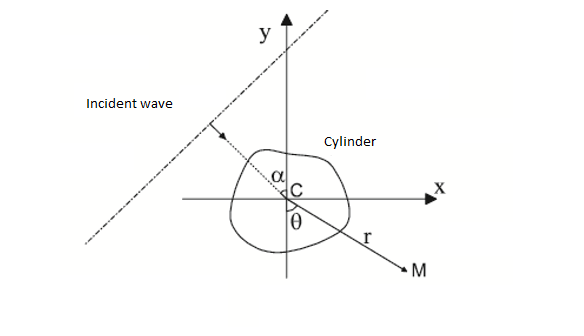
\includegraphics[scale=1,angle=0]{Images/Image2.PNG}
    \caption{General situation of the problem.}
    \label{fig:Image2}
\end{figure}

Here, $\alpha$ is the incident angle of the wave and $r$ and $\theta$ are the polar position of the point $M$. Furthermore, the center of the cylinder is at the same place as the origin. 

\section{Equations}


The wave equation can be written as follows:

\begin{equation}
 (\nabla + k^2).p = 0 
\end{equation}

In cylinder landmark, this result becomes :

\begin{equation}
 \frac{1}{r}\frac{\partial}{\partial r}(
 \frac{ r \partial p}{\partial r}) + \frac{1}{r^2}\frac{\partial^2 p}{\partial \theta^2} + \frac{\partial^2 p}{\partial z^2} + k^2 p = 0 
\end{equation}

The problem is independent of the z-dimension so we obtain :

\begin{equation}
 \frac{1}{r}\frac{\partial}{\partial r}(
 \frac{ r \partial p}{\partial r}) + \frac{1}{r^2}\frac{\partial^2 p}{\partial \theta^2} + k^2 p = 0 
\end{equation}

This problem allows us to use the separation of variables (also known as the Fourier method) and allows to rewrite an equation so that each of two variables occurs on a different side of the equation. The set of solution p can be written as:

\begin{equation}
 p(r,\theta) = R(r).\Theta(\theta)
\end{equation}

Thanks to the separation of variable, we know that we have a set of solutions which is countable so we can write:

\begin{equation}
p_{n}(r,\theta) = R_{n}(r).\Theta_{n}(\theta)
\end{equation}

The function $\Theta$ is $2\pi$ periodic so it can be written as:

\begin{equation}
\Theta_{n}(\theta) = a_{n}.e^{in\theta} + b_{n}.e^{-in\theta}
\end{equation}

Thanks to the Bessel and Hankel functions, we can express the solution:

\begin{equation}
R_{n} = c_{n}.J_{n}(kr) + d_{n}.Y_{n}(kr)
\end{equation}

Or:

\begin{equation}
R_{n} = c_{n}.H^{(1)}_{n}(kr) + d_{n}.H^{(2)}_{n}(kr)
\end{equation}

The set of solutions can be expressed by the functions:

\begin{equation}
J_{n}(kr)e^{in\theta} \qquad Y_{n}(kr)e^{-in\theta}  \qquad    n\in \mathbb{Z}
\end{equation}

\begin{equation}
H^{(1)}_{n}(kr)e^{in\theta} \qquad H^{(2)}_{n}(kr)e^{-in\theta}  \qquad    n\in \mathbb{Z}
\end{equation}

We will have two waves:
\begin{itemize}
\item An incident wave $p_{inc}$.
\item A diffused wave $p_{dif}$ resulted from the reaction of the incident wave and the object.
\end{itemize}

\chapter{Expression of the wave resulting from this situation.}

Both the incident wave and the diffused wave have to be defined at (0,0) and mustn't diverge when $r\rightarrow +\infty$.

The consequences are that the incident wave can be written as :

\begin{equation}
p_{inc} =  	\sum_{n=-\infty}^{\infty} a_n J_{n}(kr)e^{in\theta} 
\end{equation}

If we choose to use the Hankel functions in order to express the diffused wave, we get the result:

\begin{equation}
p_{dif} =  	\sum_{n=-\infty}^{\infty} b_{n}H^{(1)}_{n}(kr)e^{in\theta}
\end{equation}

The limit condition which applies here is the SOMMERFELD condition. That means that:

\begin{equation}
p_{inc}(r,\theta) = p_{dif}(r,\theta) \qquad \forall(r,\theta) \in \{Border\, of\, the\, object\}
\end{equation}

Thanks to the fact every term are independent, we have:

\begin{equation}
b_{n}.H^{(1)}_{n}(kr) = a_n J_{n}(kr) \qquad \forall n \in \mathbb{N} \qquad \forall(r,\theta) \in \{Border\, of\, the\, object\}
\end{equation}

So we have a relation between the coefficient $a_n$ and $b_n$. We still have to find an expression for $a_n$.

The wave $p_{inc}$ is a plane wave which means that it can be write as:

\begin{equation}
p_{inc} = e^{i k_{inc} x} \qquad or \qquad p_{inc} = e^{i k_{inc} r.\cos( \theta - \alpha )}
\end{equation}

If we develop the term $\cos(\theta-\alpha)$ as a Fourier series, we get the equation:

\begin{equation}
p_{inc} =  	\sum_{n=-\infty}^{\infty} i^n e^{-i n \alpha} J_{n}(kr)e^{in\theta} 
\end{equation}

Which means $a_n = i^n e^{-i n \alpha} $. With this, we can express the wave result from the diffraction of the incident wave on the object.

\chapter{Examples of situations encountered.}

During this project, we will have only two situations.

We will in a first step consider a unique  cylinder which radius changes through time and we will study the magnetic field at the point M:

\begin{figure}[H]
\centering
    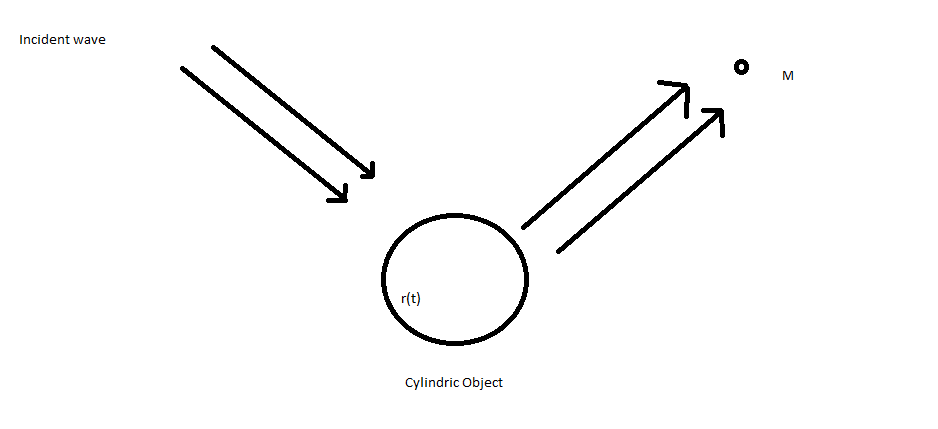
\includegraphics[scale=0.6,angle=0]{Images/Image3.png}
    \caption{Study with a unique object.}
    \label{fig:Image3}
\end{figure}

In a second step, we will consider a lot of cylinders which can move through time and study the magnetic field at the point M: 

\begin{figure}[H]
\centering
    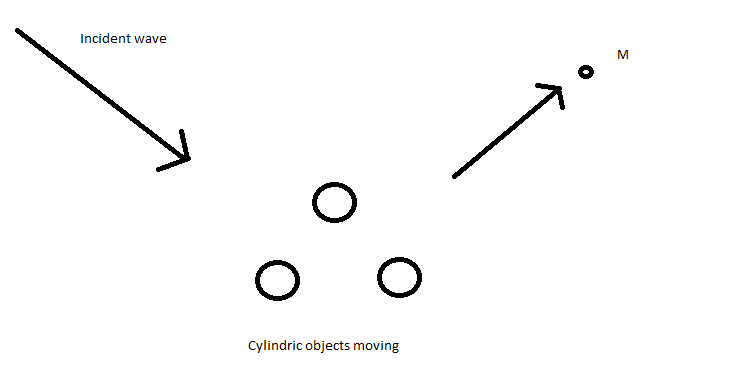
\includegraphics[scale=0.6,angle=0]{Images/Image4.png}
    \caption{Study with a set of objects.}
    \label{fig:Image4}
\end{figure}

For this situation, we have to estimate the phase shift between those objects and an origin. Thanks to some geometric theorems, this can be easily obtained. 


\bigskip

\chapter*{Conclusion}
The code needed in order to generate these signals is already working and all we need is to simulate the movement and the deformation of one or two cylinders and see the effect of the movement and the form deformation on the electromagnetic signature.

You will have to use the script Objectdiff.py in order to generate a signal.

%----------------------------------------------------------------------------------------
%	PART II 
%----------------------------------------------------------------------------------------
\part{Time/frequency analysis}

\chapter{Spectrogram}

The spectrogram is the most common tools used in order to do a time frequency representation. This representation use the short-time-Fourier transformation in order to apply an fast-Fourier transformation on a slippery window of the signal. In the end, we get an image which represent the frequency which compose the signal at an instant t given.

Let consider the signal chirp below which correspond to a signal which its frequency increases from 0 to 300Hz.

\begin{figure}[H]
\centering
    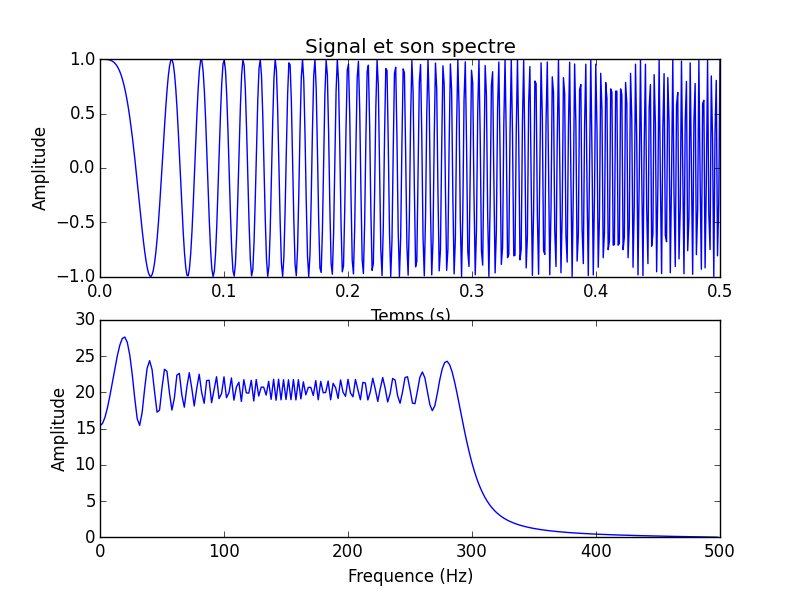
\includegraphics[scale=0.6,angle=0]{Images/ChirpTF.png}
    \caption{Time and frequency representation of a chirp signal.}
    \label{fig:ChirpTF}
\end{figure}

The figure below shows the results we can get:

\begin{figure}[H]
\centering
    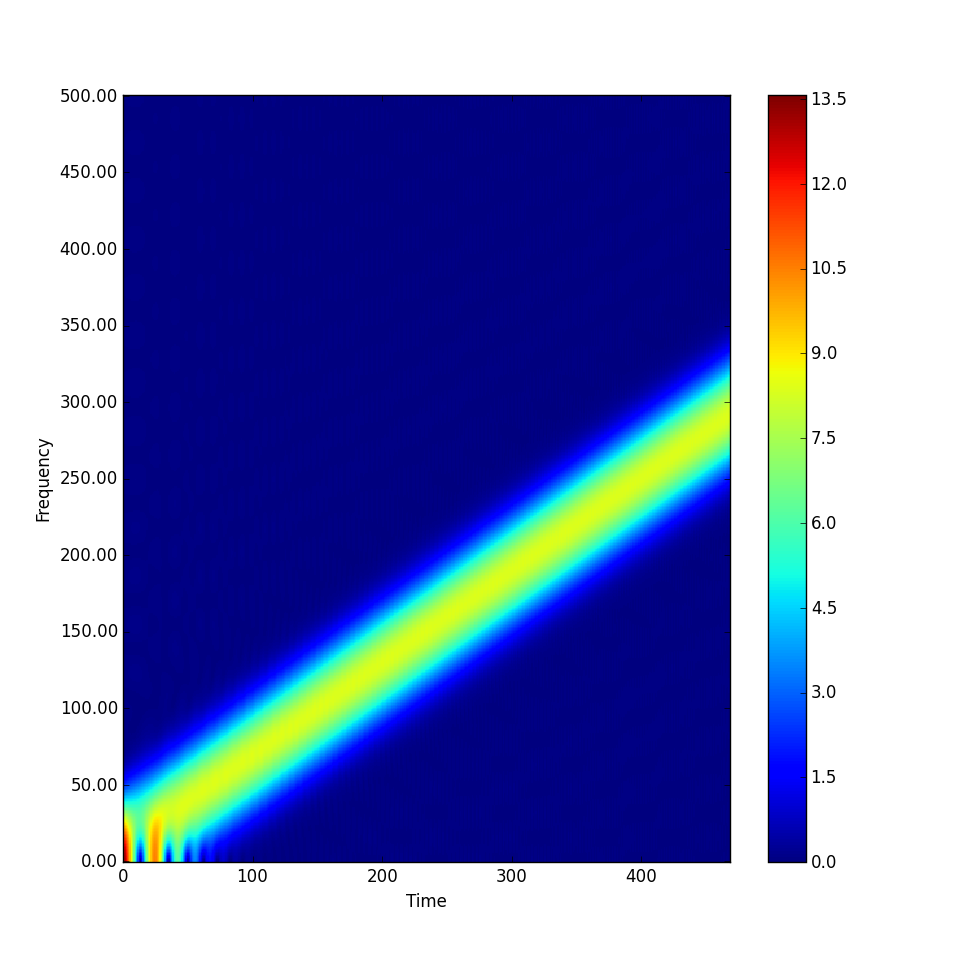
\includegraphics[scale=0.6,angle=0]{Images/Chirp_STFT.png}
    \caption{STFT/spectrogram of a chirp signal.}
    \label{fig:Chirp_STFT}
\end{figure}

This figure shows clearly that the frequency of the signal increass through time but the result is a little blur and isn't very accurate.

\chapter{Wigner-Ville}

The Wigner-Ville distribution allows us to get a far more accurate time frequency representation. Nevertheless, this distribution create some interferences if the signal is a combination of different frequency laws.

The Wigner-Ville Distribution (WVD) of a signal y(t), denoted by $W_z(t,f)$, is defined as :

\begin{equation}
W_z(t,f) = \int_{n=-\infty}^{\infty} z ( t + \tau / 2 ) z^* (t - \tau / 2) e^{-j 2 \pi f \tau} d \tau
\end{equation}

The following figure shows the result of the Wigner-Ville representation on the previous signal:

\begin{figure}[H]
\centering
    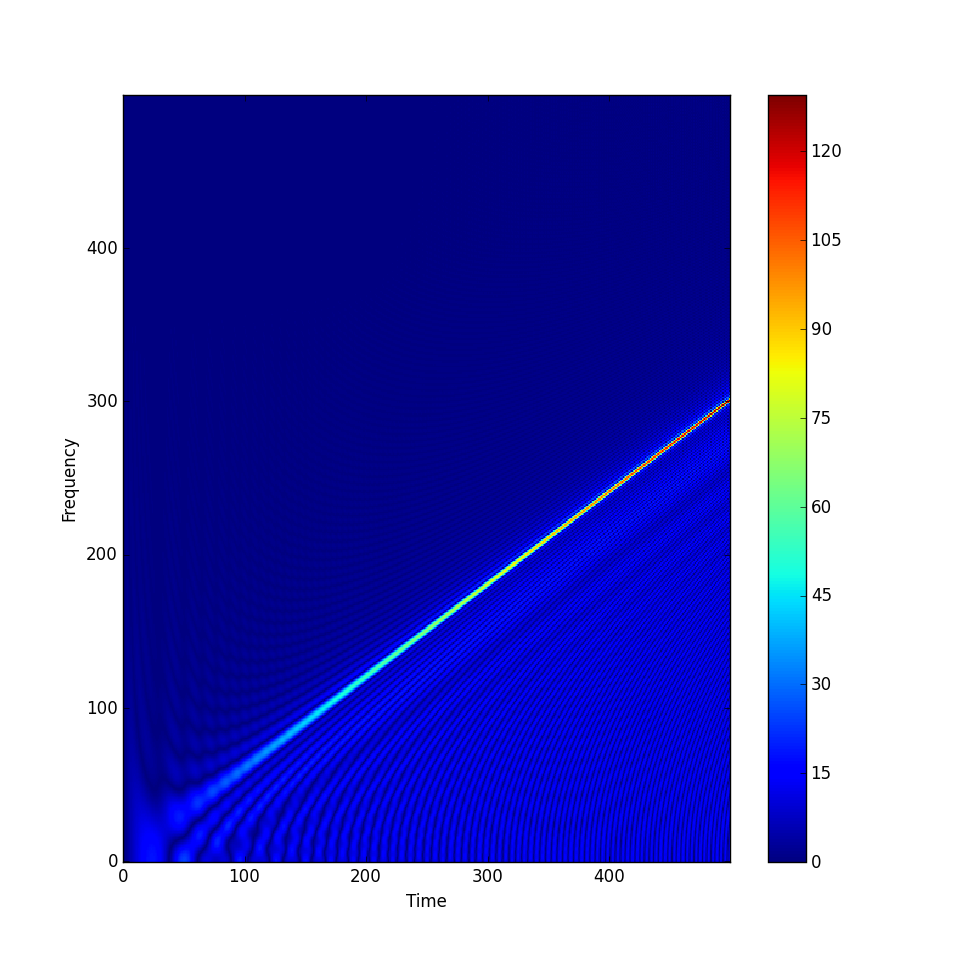
\includegraphics[scale=0.5,angle=0]{Images/Chirp_WV.png}
    \caption{Wigner-Ville of a chirp signal.}
    \label{fig:Chirp_WV}
\end{figure}

Nevertheless, if we consider the following signal which contains two sinusoids, with different frequency and with one which last for only a portion of the signal. We get the result below:

\begin{figure}[H]
\centering
    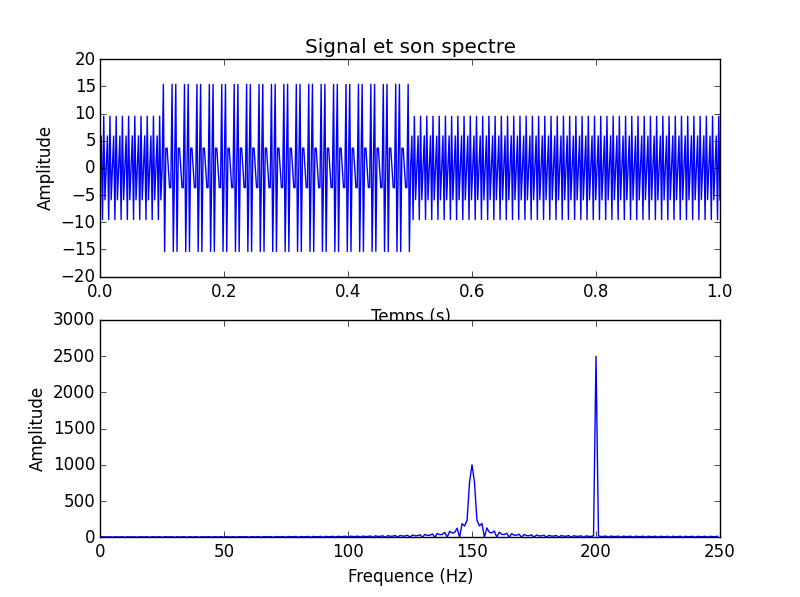
\includegraphics[scale=0.5,angle=0]{Images/SignalSimple.png}
    \caption{Time and frequency representation of the signal with two frequency laws.}
    \label{fig:SignalSimple}
\end{figure}

\begin{figure}[H]
\centering
    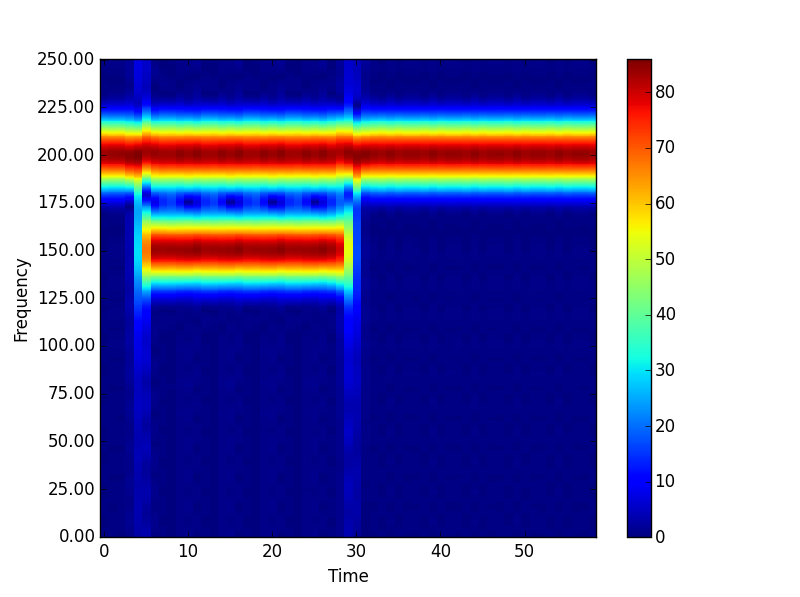
\includegraphics[scale=0.5,angle=0]{Images/figure_6STFT.png}
    \caption{Spectrogram of the signal.}
    \label{fig:SignalSimple_Spectrogram}
\end{figure}

\begin{figure}[H]
\centering
    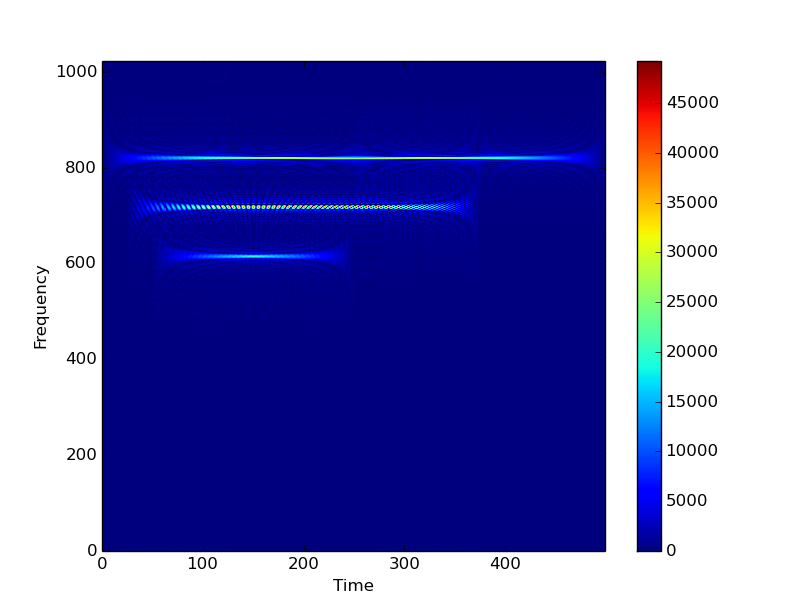
\includegraphics[scale=0.5,angle=0]{Images/SignalSimple_WV.png}
    \caption{Wigner-Ville of the signal.}
    \label{fig:SignalSimple_WV}
\end{figure}

As you can see, there are an interference which imply to analyse this figure if we want to extract relevant information.

\textbf{NB :} The differences in the frequency scale is due to a problem in the implementation I realized. I will correct this as soon as I can.

\chapter{Pseudo Smooth Wigner-Ville}

The  Pseudo-Wigner-Ville Distribution is defined as:

\begin{equation}
W_z(t,f) = \int_{n=-\infty}^{\infty} h ( \tau ) z ( t + \tau / 2 ) z^* (t - \tau / 2) e^{-j 2 \pi f \tau} d \tau
\end{equation}

where $h$ is a regular window. This windowing is equivalent to a frequency smoothing of the WVD so It leads to the attenuation of the interference terms but it will damage the signal representation.

The result for the previous signal is below:

\begin{figure}[H]
\centering
    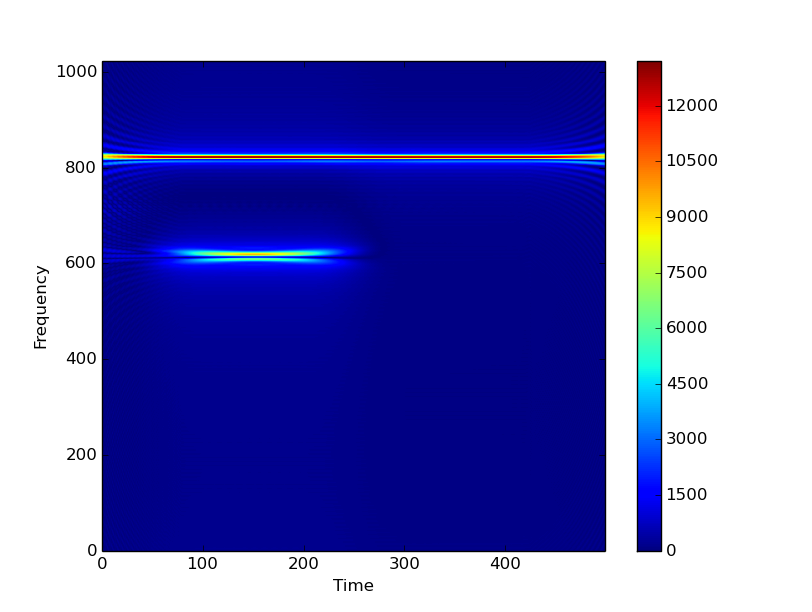
\includegraphics[scale=0.5,angle=0]{Images/SignalSimple_PSWV.png}
    \caption{Pseudo Smooth Wigner-Ville of the signal.}
    \label{fig:SignalSimple_PSWV}
\end{figure}

\chapter*{Conclusion}
\bigskip
All those representations present some interests or disadvantages. Nevertheless, if we want to get as much information as we can, we will need to switch between a representation to another according to the kind of signal we have. At the beginning of the project, an implementation of the Flandrin library coming from Matlab was implemented but we found afterwards a python library which was already doing this part. The following link shows the function of this library and the second one explain how it can be install on your computer. The previous pictures came from our own functions but the next pictures will use the function of this library.

\medskip

\textit{https://github.com/scikit-signal/pytftb}

\medskip

\textit{http://pytftb.readthedocs.org/en/master/}

\medskip

All the time frequency representation of this project now use those function which provide a much more reliable result than the function we tried to implemented.


%----------------------------------------------------------------------------------------
%	PART III 
%----------------------------------------------------------------------------------------

\part{Time frequency analysis}



\chapter{Seam carving algorithm}

For this part, most of the tools come from those references \cite{Doopler1} \cite{Doopler2} \cite{Doopler3}.
\textbf{For now, I'm still working on this part so I will complete this part as soon as I get result.}
The main purpose of this article is to present an algorithm which allow us to find the speed of an object thanks to the Doppler effect but it can be use here in order to find the frequency laws which compose the signal. With this, we have a way to find correlation between the electromagnetic signature and the kind of from changes of an object.


\chapter{Application on our project}

We will now apply this algorithm to the time frequency representation coming from the part 2 and from the signal generate in the part 1.
\textbf{For now, I'm still working on this part so I will complete this part as soon as I get result.}




\appendix
\part{Appendix}
\chapter*{Gaant diagram}

\begin{figure}[H]
\centering
    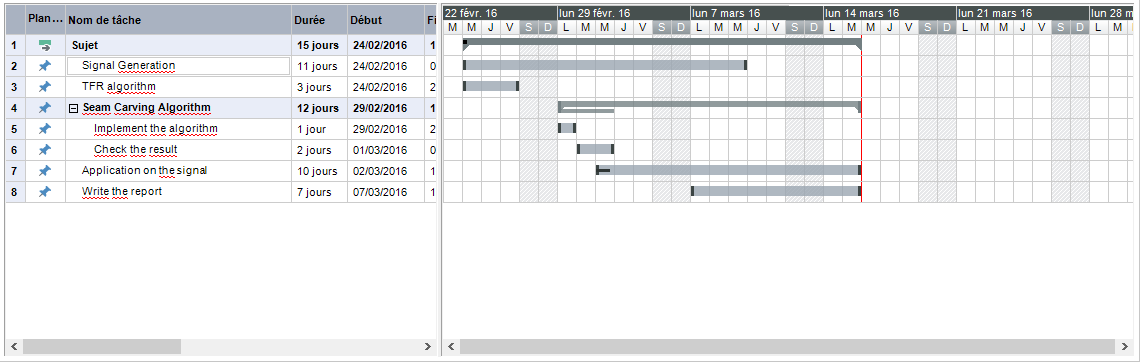
\includegraphics[scale=0.6,angle=0]{Images/GaantV2.PNG}
    \caption{Gaant diagram.}
    \label{fig:GaantV1}
\end{figure}

There are a lot of differences between what I expected and what I have done. I had to do a lot of verification in order to check if the code which generate the signal was correct. The seam carving was implemented pretty quickly but the time-frequency representation didn't give the result expected and it took me a lot of time.

The program which has been used in order to generate this diagram is \textbf{MindView 6.0}

%----------------------------------------------------------------------------------------
%	BIBLIOGRAPHIE
%----------------------------------------------------------------------------------------

%\addcontentsline{toc}{part}{Bibliography}
%\bibliographystyle{apalike-fr}
\bibliographystyle{plain}
\bibliography{bibliographie}


%----------------------------------------------------------------------------------------

\end{document}